\chapter{MAD-F Evaluation}
\label{chapter:Chapter 5}
\lhead{Chapter 5. \emph{MAD-F Evaluation}}

In this Chapter, we present a group of experiments on the MAD-F capabilities. Firstly, we undertake data ingestion and storage performance test, which is followed by a exploratory analysis of the gathered data. Secondly we validate each of the ADS modules, starting with the RB-ADS Experiment, where the data that was collected previously is Experiment is injected in this module with the help of a simulator. After an Experiment over the ADS is conducted, where for each of the anomalies that are detected we provide and exploratory analysis of the results.
The \emph{validation} of the results presented in this Chapter, can only truly be done by Maritime Officer. What is to be called as anomalies in this work must not be interpreted as an actual maritime illegality, but only as a possible anomaly, which needs always to be validated by Maritime Officer. The real validation of the developed MAD-F will be done by the project end-users the Maritime Experts. \textsc{Marisa} being an highly collaborative and undergoing project, such validation at the time of writing this dissertation were still to occur. The validation of the MAD-F by the project end users is described under in Section~\ref{Section: 5 Marisa Validation}. 
All the experiments under in this Chapter were conducted on a Desktop PC using a Intel Core I5-7600k CPU with 16Gb of RAM.

\section{Data Ingestion Experiment}
\label{section: Experiment Data}
Data Ingestion Experiment refers to the Experiment were we accessed the performance of the Data-Ingestion capability of MAD-F. In order to achieve this, we provided a real NMEA feed as input to our the Data Ingestion Module. The NMEA feed was provided by the Portuguese Navy via the \textsc{Marisa} project, and this specific feed aggregated messages from multiple antennas around Portugal.
 
With the provided feed, we allowed the MAD-F to be executed for five straight days, thus ingesting pre-processing and wrangling the NMEA feed into Behavioural Points. As for this experiment we used a real NMEA feed, the messages were firstly decoded into a readable format, and only then after the whole pre-processing was done, the $BPs$ were stored in the Trajectory Extraction Cassandra Data-Base.

From the 5 days of data acquiring, we acquired from a total of $2,259,615~BPs$ from $5,563$ different Vessels.
As the provided feed did not broadcast any vessel static information, from the vessel that generated each message. The vessel static information namely the vessel type and country of origin, were scrapped from the internet using the developed \emph{Vessel Type Scrapper} which we presented in Section~\ref{subsection: Vessel Type}. 
From the $5,563$ vessels, $6$ of them were not considered for this Experiment. The MMSI of this vessels was either not found or their MMSI was representative for more than one Vessel. The latter, represents an abnormal situation which could be denominated Spoofing, as represented by the authors in~\cite{Ray2015DeAISRisks} or in \footnote{http://globalfishingwatch.org/data/spoofing-one-identity-shared-by-multiple-vessels}. This is a occurring problem when handling AIS data, and will be discussed in the future work.
In Figure~\ref{fig: 5 Vessel Type Distribution}, we present the vessel type distribution from the acquired $BPs$.
\begin{figure}[H]
	\centering
	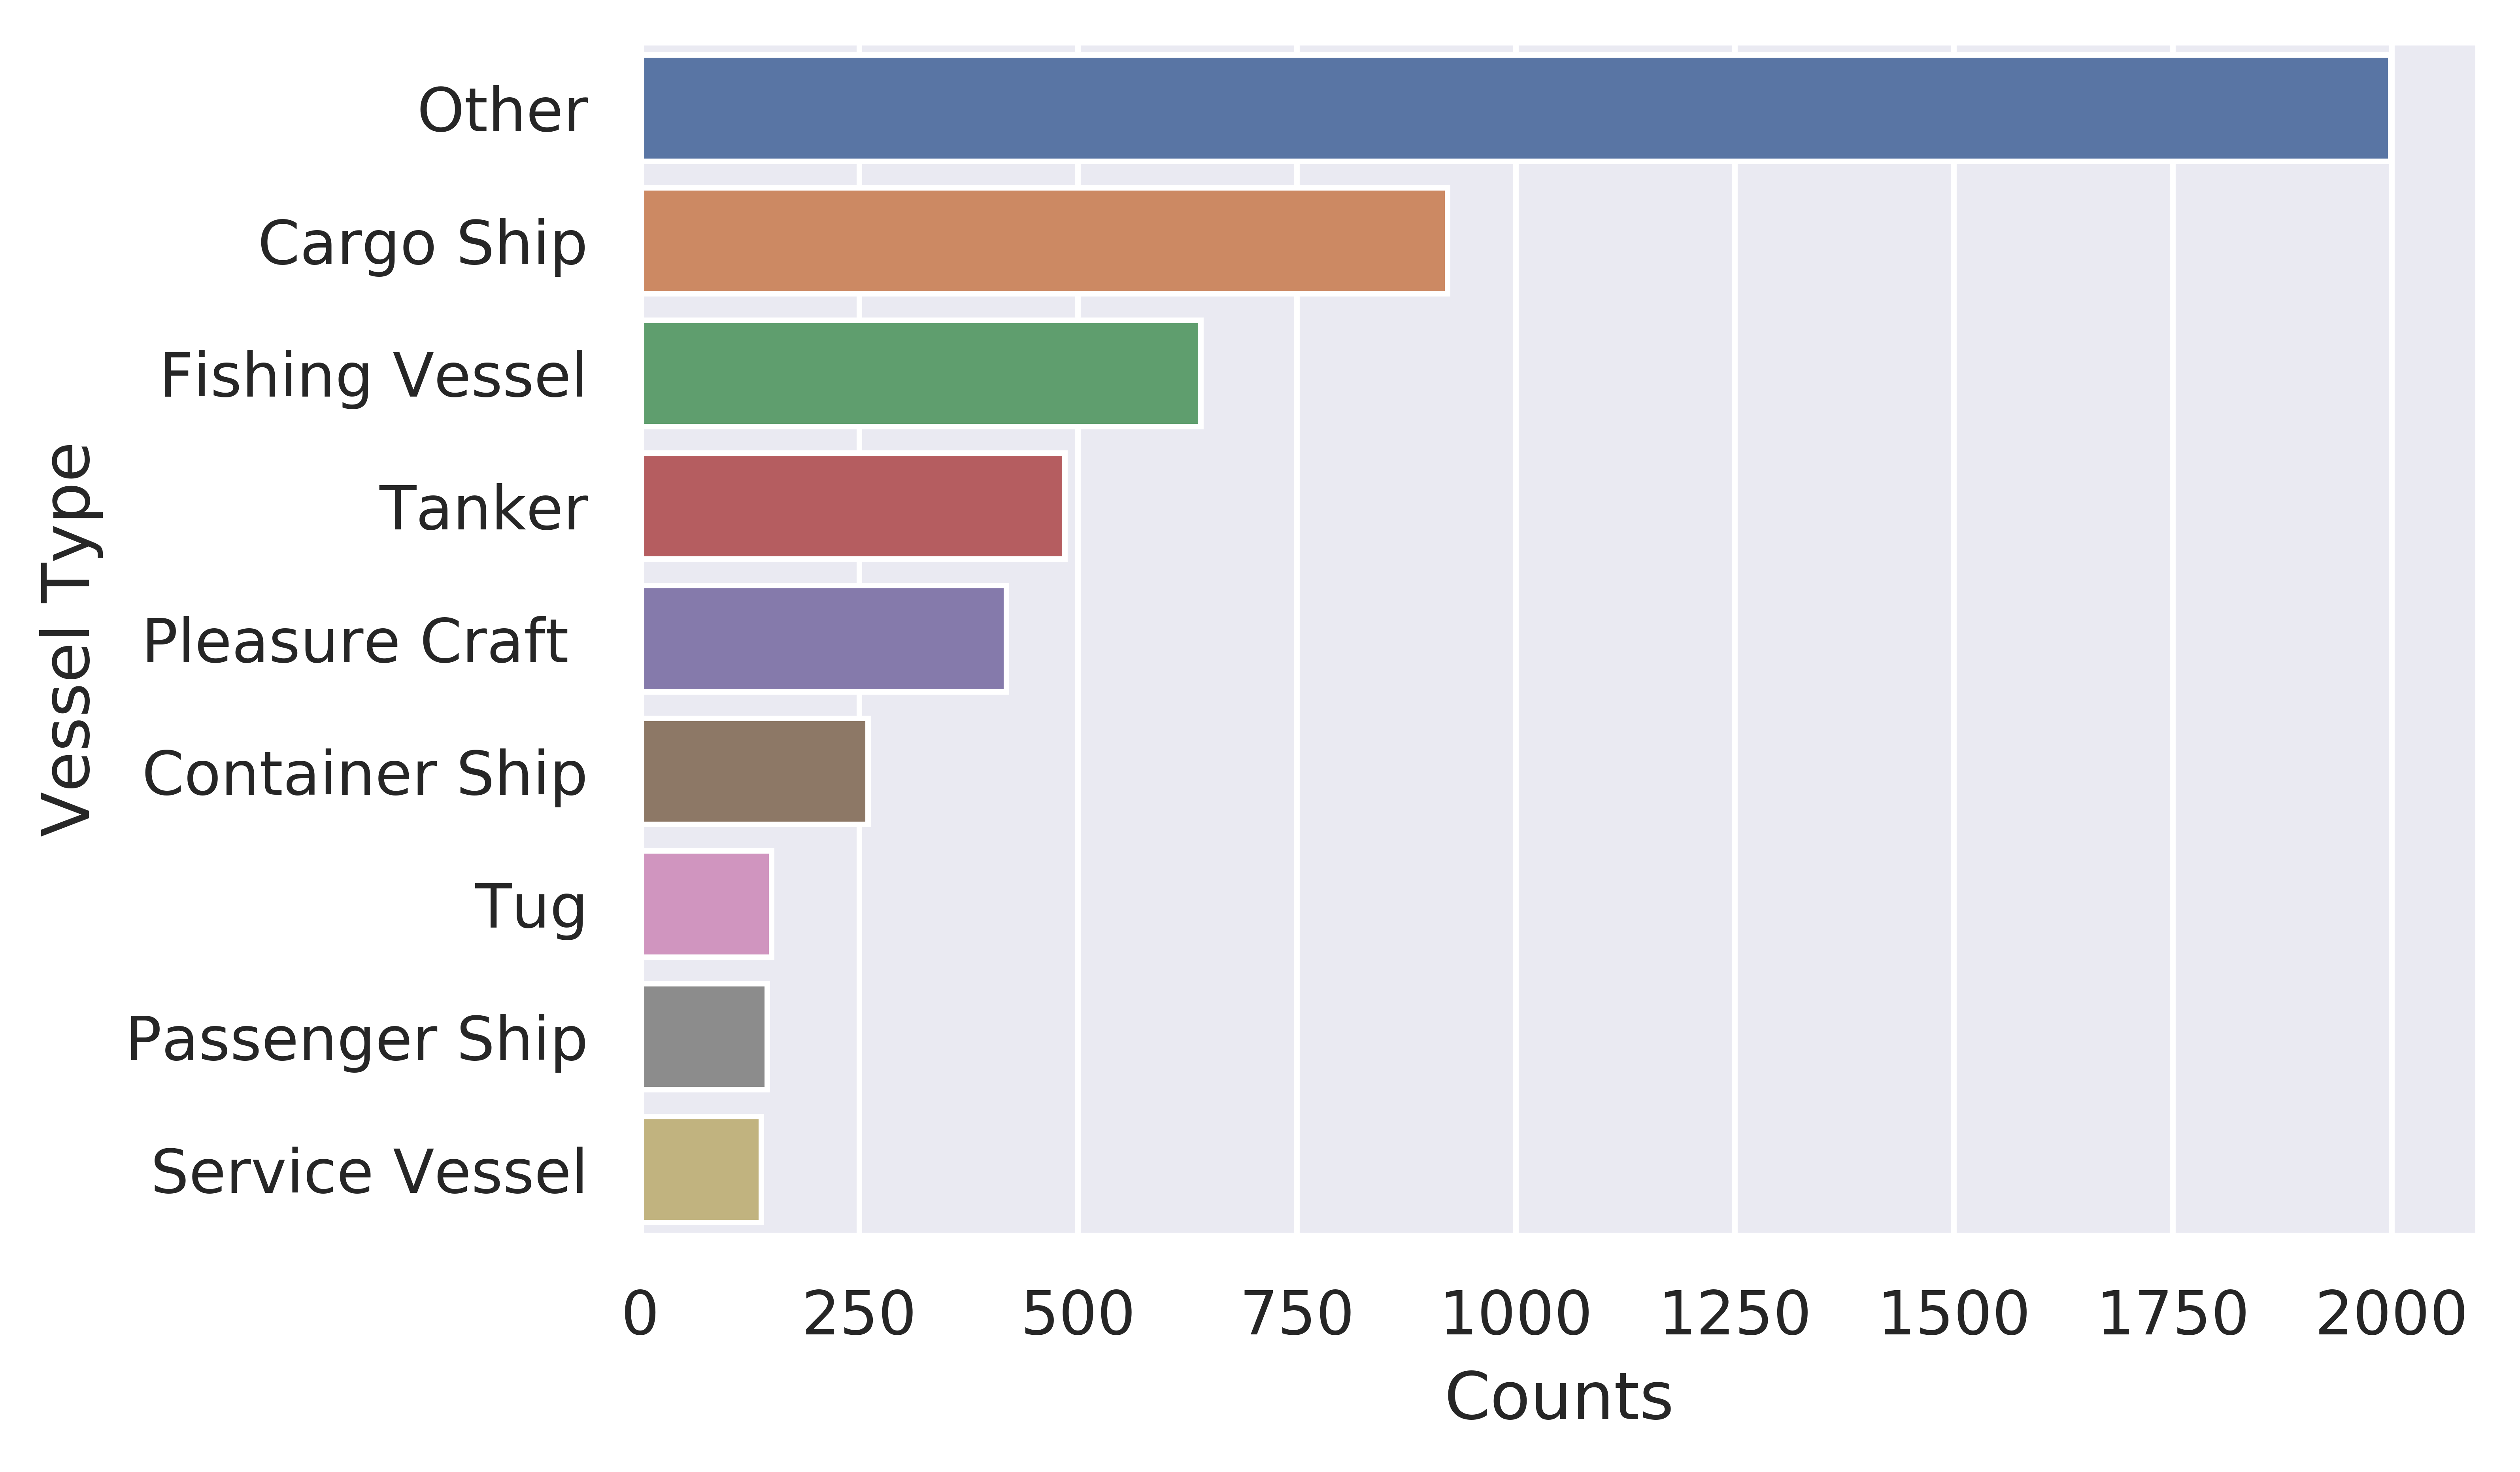
\includegraphics[scale = .7]{figures/Ch5/DataValidationVesselType.png}
    \caption{Vessel Type distribution of $5,157$ Vessels.}
    \label{fig: 5 Vessel Type Distribution}
\end{figure}

Another feature calculated while transforming data into $BPs$ was the point-based closest distance to coast and ports, which was done to every received NMEA AIS message received. In order to validate if this calculation were in fact being accurate, we analysed based on the received $BPs$ which countries were the closest and the respective ports.
In Table~\ref{Table: 5 Closest Countries} we present the distribution of closest countries. 
\begin{table}[H]
\centering
\caption{Most Frequent Closest Countries Counts.}
\label{Table: 5 Closest Countries}
\begin{tabular}{@{}lcc@{}}
\toprule
Country & Counts & Counts(\%) \\ \midrule
Spain & 1,306,436 & 58\% \\
Portugal & 663,841 & 29\% \\
Morocco & 259,776 & 11\% \\
Gibraltar & 26,885 & 1\% \\
France & 2,516 & 0.1\% \\ \bottomrule
\end{tabular}
\end{table}
In Table ~\ref{Table: 5 Closest Ports} we present a post validation of the closest Ports for every received message. This was done as a way to analyse if based on the the closest country the most closest ports seems plausible, as a individual message validation would be impossible. Thus, under we present a subset of top most frequent closest ports from the $69$ total possible Ports found in the data.
\begin{table}[H]
\centering
\caption{Most Frequent Closest Ports Counts.}
\label{Table: 5 Closest Ports}
\begin{tabular}{@{}lcc@{}}
\toprule
Port Name & Counts & Counts(\%) \\ \midrule
Lisboa & 142,464 & 6,3\% \\
Villa Garcia De Arosa & 112,254 & 5\% \\
Europa Point(Gibraltar) & 109,273 & 4,8\% \\
Lagos & 107358 & 4,7\% \\
Las Palmas & 106,116 & 3,5\% \\
Cadiz & 79,577 & 3,5\% \\
La Corunha & 78,929 & 3,5\% \\
Malaga & 65,227 & 2,9\% \\
Vigo & 64,759 & 2,9\% \\
Faro & 62,925 & 2,9\% \\ \bottomrule
\end{tabular}
\end{table}

By displaying all the 2.2 Million $BPs$ into a density plot, we try to positional occurrence of the transmitted messages. As scattering Millions of points is computational heavy, and if "normal" plotting packages were to be used not possible with the Hardware specifications presented in the begining of this Chapter. Thus the density plots presented in this Chapter were using the~\footnote{http://vaex.astro.rug.nl}, which is optimised huge datasets. 

\begin{figure}[H]
	\centering
	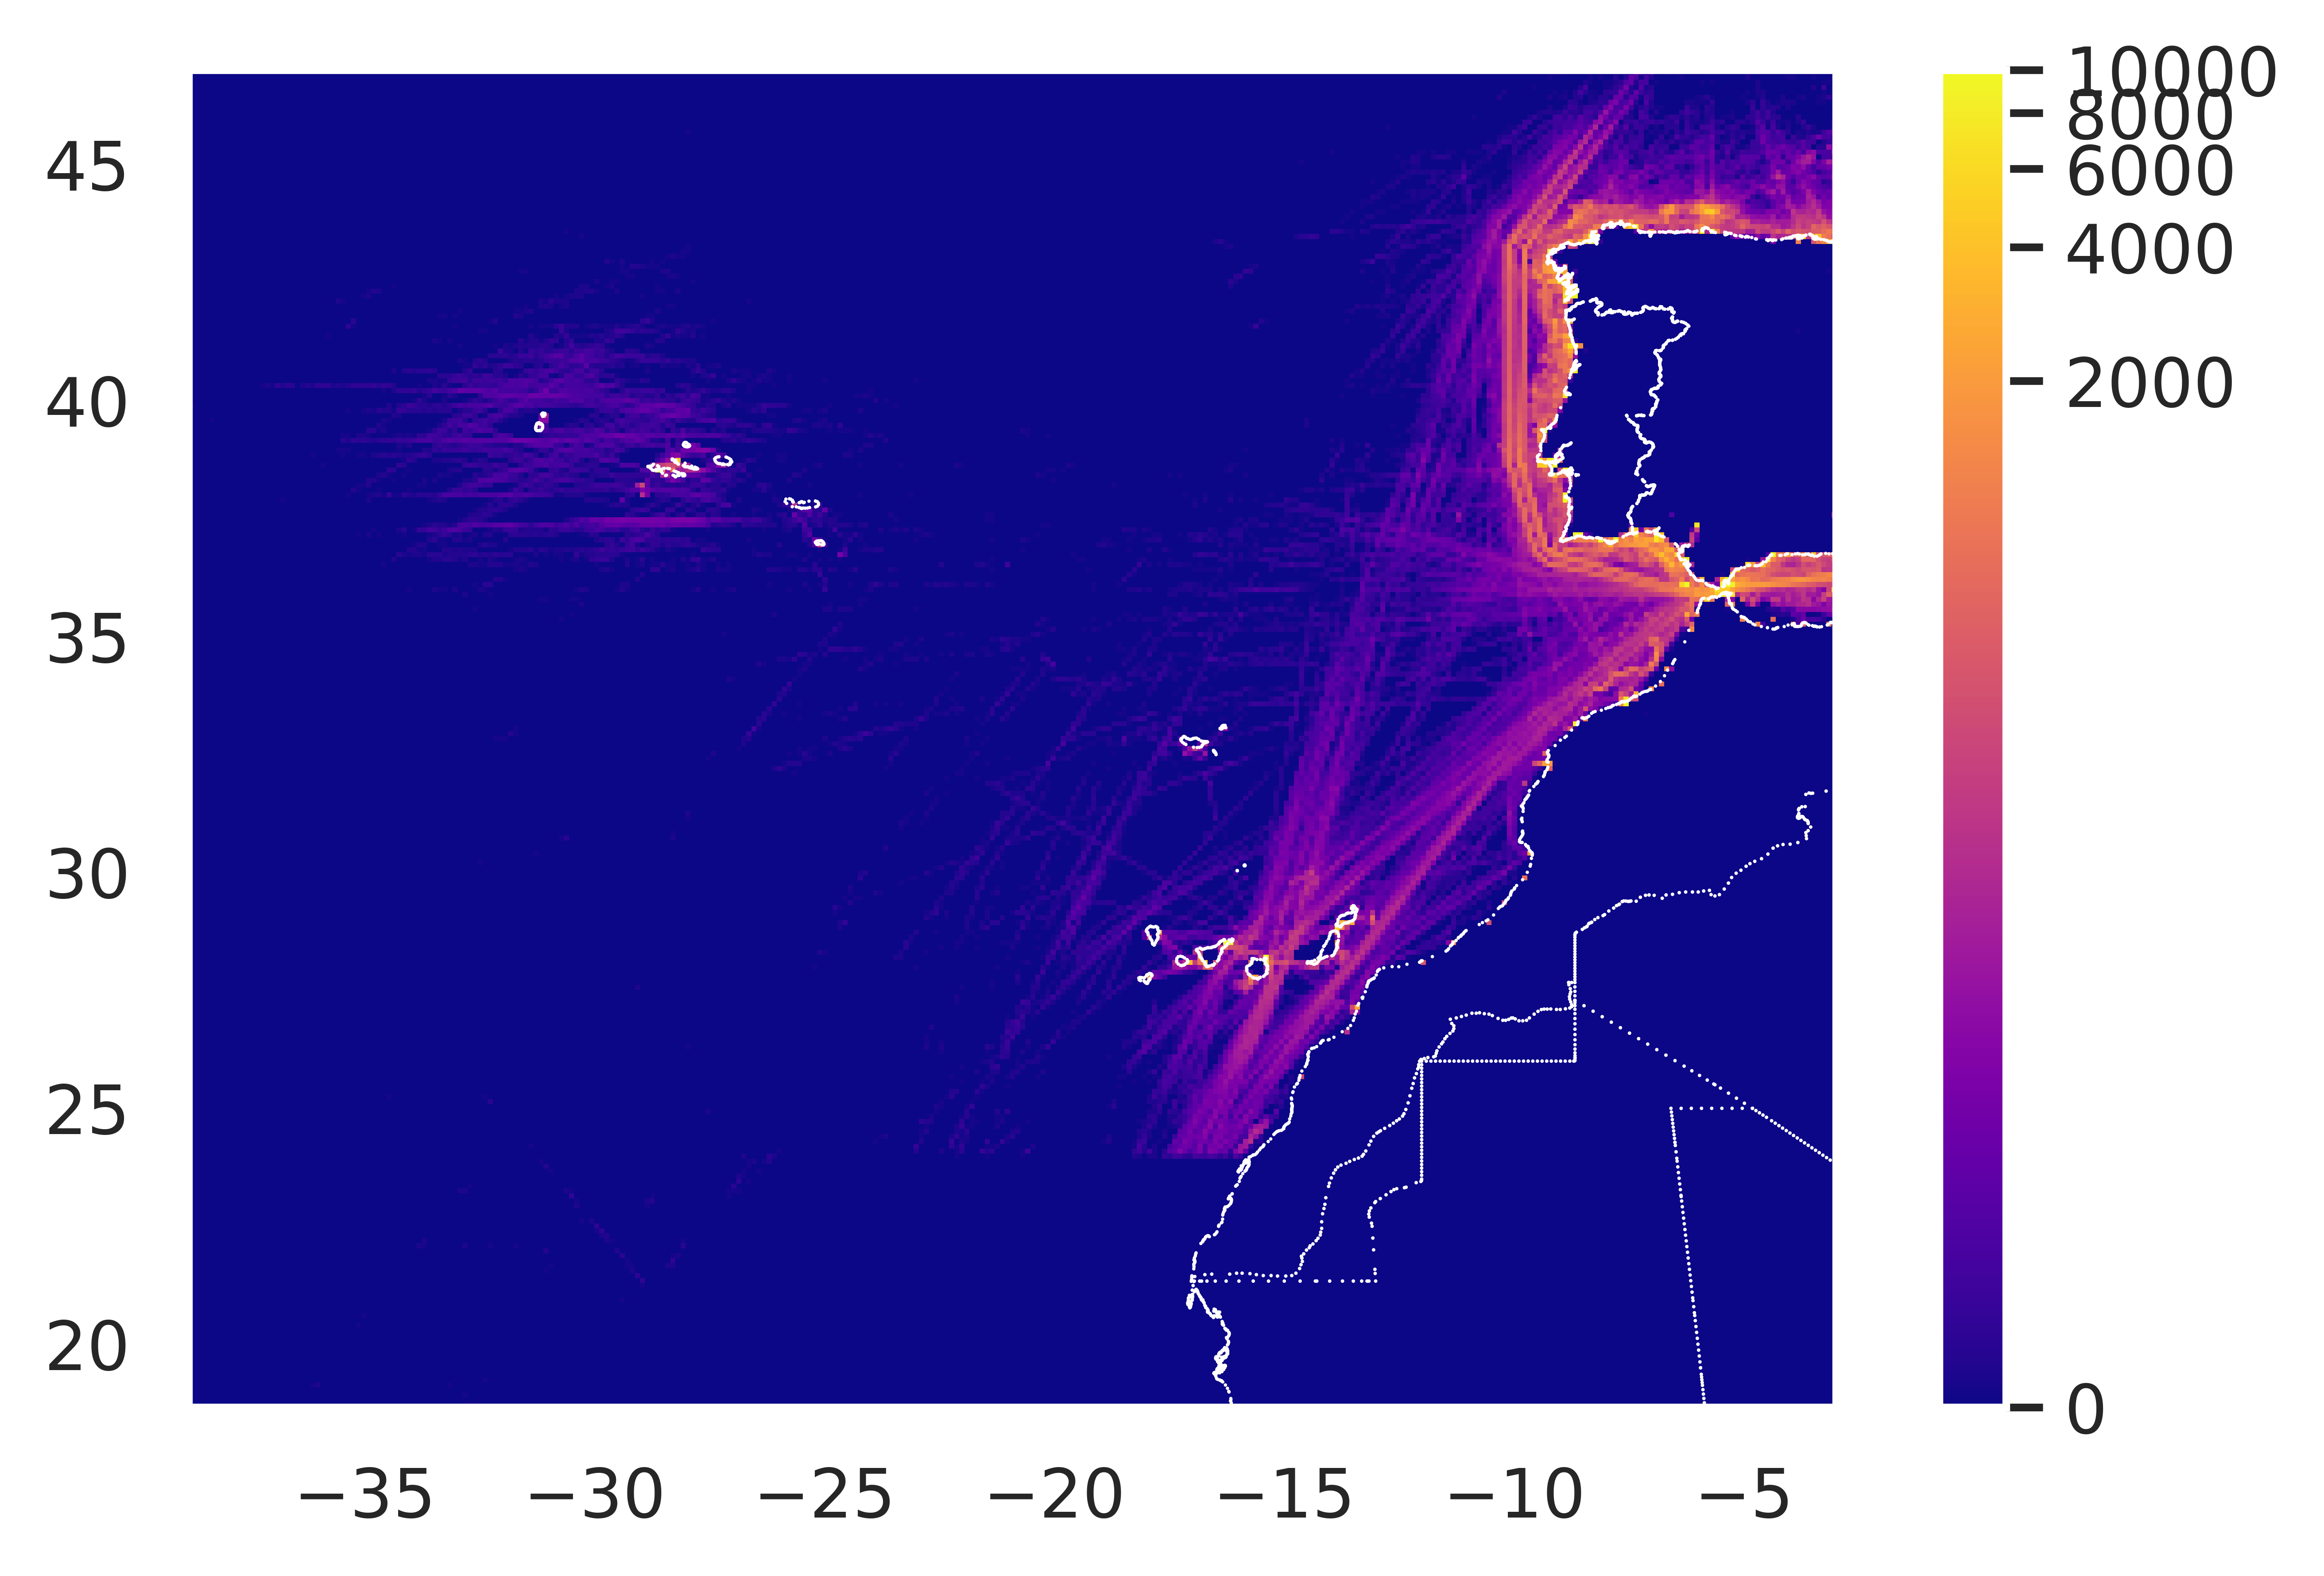
\includegraphics[width=\textwidth]{figures/Ch5/ThesisExpDensity.png}
    \caption{Density map, with all the approximately
    $2.2$ Million points.}
    \label{fig: 5 Exp1DensityMap}
\end{figure}

What we found by analysing Figure~\ref{fig: 5 Exp1DensityMap} is that in fact the messages that were received via the Portuguese Navy antennas. Which explains the reception of messages near the Madeira and Azores islands.  What is possible also to analyse in the Figure, is nearby the Portuguese coastal line a few lines of high density traffic show up. These lines represent the navigational lanes, and when navigation in this lanes vessels tend to have a more standardised behaviour. Such fact can be explored other types of AD, and is presented by the authors in~\cite{Yan2016} and~\cite{Silveira2013UsePortugal}. The acknowledge of this lanes for anomaly detection will be endorsed in future work.


\section{RB-ADS Experiment}
\label{section: RB-ADS Experiment}
This experiment was conducted, in order to validate the real time capacities of the RB-ADS Module. In order to validate such capacities, we focused this experiment on the validation by analysis of the anomalies which were generated, and whether this anomalies were generated in near-real time.
This experiment was simultaneously conducted as the previous Experiment~\ref{subsection: Data Ingestion}. This was possible as the incoming messages after being ingested and pre-processed they were stored in the Trajectory Extraction module as $BPs$ but simultaneously the same $BPs$ were inputted in the RB-ADS module.
The RB-ADS module managed the incoming $BPs$, using the implemented service queue, which we explained in~\ref{section: 4 Rule Based Anomaly Detection}. For this experiment we set the service queue $N$, size to \textbf{$2$}. This made the anomaly detection be executed, if any vessel queue had two $BPs$, with the set of rules, which we defined and are represented under in Table~\ref{Table: 5 exp. RB-ADS rules}. 

\begin{table}[H]
\centering
\caption{RB-ADS Experiment, rule configurations, where the columns represent the variables.}
\label{Table: 5 exp. RB-ADS rules}
\begin{tabular}{@{}ccccc@{}}
\toprule
Rule & SOG variation & GOG variation & SOG min. & Time Elapsed \\ \midrule
R1 & - & - & - & 15min. (post.) \\
R2 & \textgreater{}15 knot & - & - & - \\
R3 & - & \textgreater 25º & \textgreater 0.5 knot & - \\ \bottomrule
\end{tabular}
\end{table}

From the 5 days of executing the MAD-F, as mentioned in Section~\ref{section: Experiment Data} a total of $2,259,615 BPs$ were processed and ingested in the RB-ADF modules. With the presented set of rules a total of $191,481$ anomalies were generated. These number of anomalies is rather large, representing approximately $8\%$ of all the $BPs$ were considered anomalous for one of these rules. In Table~\ref{Table: 5 exp. results rules} we detail more explicitly the total number of anomalies by analysing the rules which generated such anomalies. As well as the matching the defined rules for this Experiment with the anomaly requirements, which were defined in~\ref{section: Framework Requirements}.

\begin{table}[H]
\centering
\caption{Anomalies found for each Rule with the respective Anomaly Requirement.}
\label{Table: 5 exp. results rules}
\begin{tabular}{@{}ccccc@{}}
\toprule
Rule & R1 & R2 & R3 & Total \\ \midrule
Count & 82,866 & 2,144 & 106,471 & 191,481 \\
\begin{tabular}[c]{@{}c@{}}Anomaly\\ Requirement\end{tabular} & AR3 & AR2 & AR1 & - \\ \bottomrule
\end{tabular}
\end{table}

From the results presented above what is possible to analyse, is that the most occurring anomaly was the abnormal change of direction this despite the filtering of normal course variations on vessels which were stopped. We further analysed the time difference between same vessel transmissions. What we found out was that the \emph{mean transmission rate}, was of approximately \textbf{10min.}, which is high for a real AIS feed. Although, if the $BPs$ which were considered anomalous from the $R1$, were not considered for the calculation of this mean, the \emph{mean transmission rate} would be \textbf{5min.}. Thus, if a new rule were to be applied where from the $R3$ only messages that had been transmitted with a time difference inferior to 5 minutes, which could be represented as  $COG.diff>25~and~TimeDiff.<5minutes$, only \textbf{7} anomaly occurrences would occur.

The additional rule presented above, was not validated with the live NMEA feed, as this was a live stream. Nevertheless, this rule was still validated with the same data. As the results from the Experiment~\ref{section: Experiment Data} were stored in the trajectory data-base, these could be accessed multiple times. For the purpose of these current work we developed a $BPs$ simulator which from the stored trajectories would simulate the real reception of AIS streams (from the perspective of the RB-ADS module).

The simulator gathers $BPs$ from the trajectories (or a group of) stored in the trajectory data-base, and send this $BPs$ to the RB-ADS, as presented in~\ref{fig: 5 BPs Simulator}.
\\
\begin{figure}[H]
	\centering
	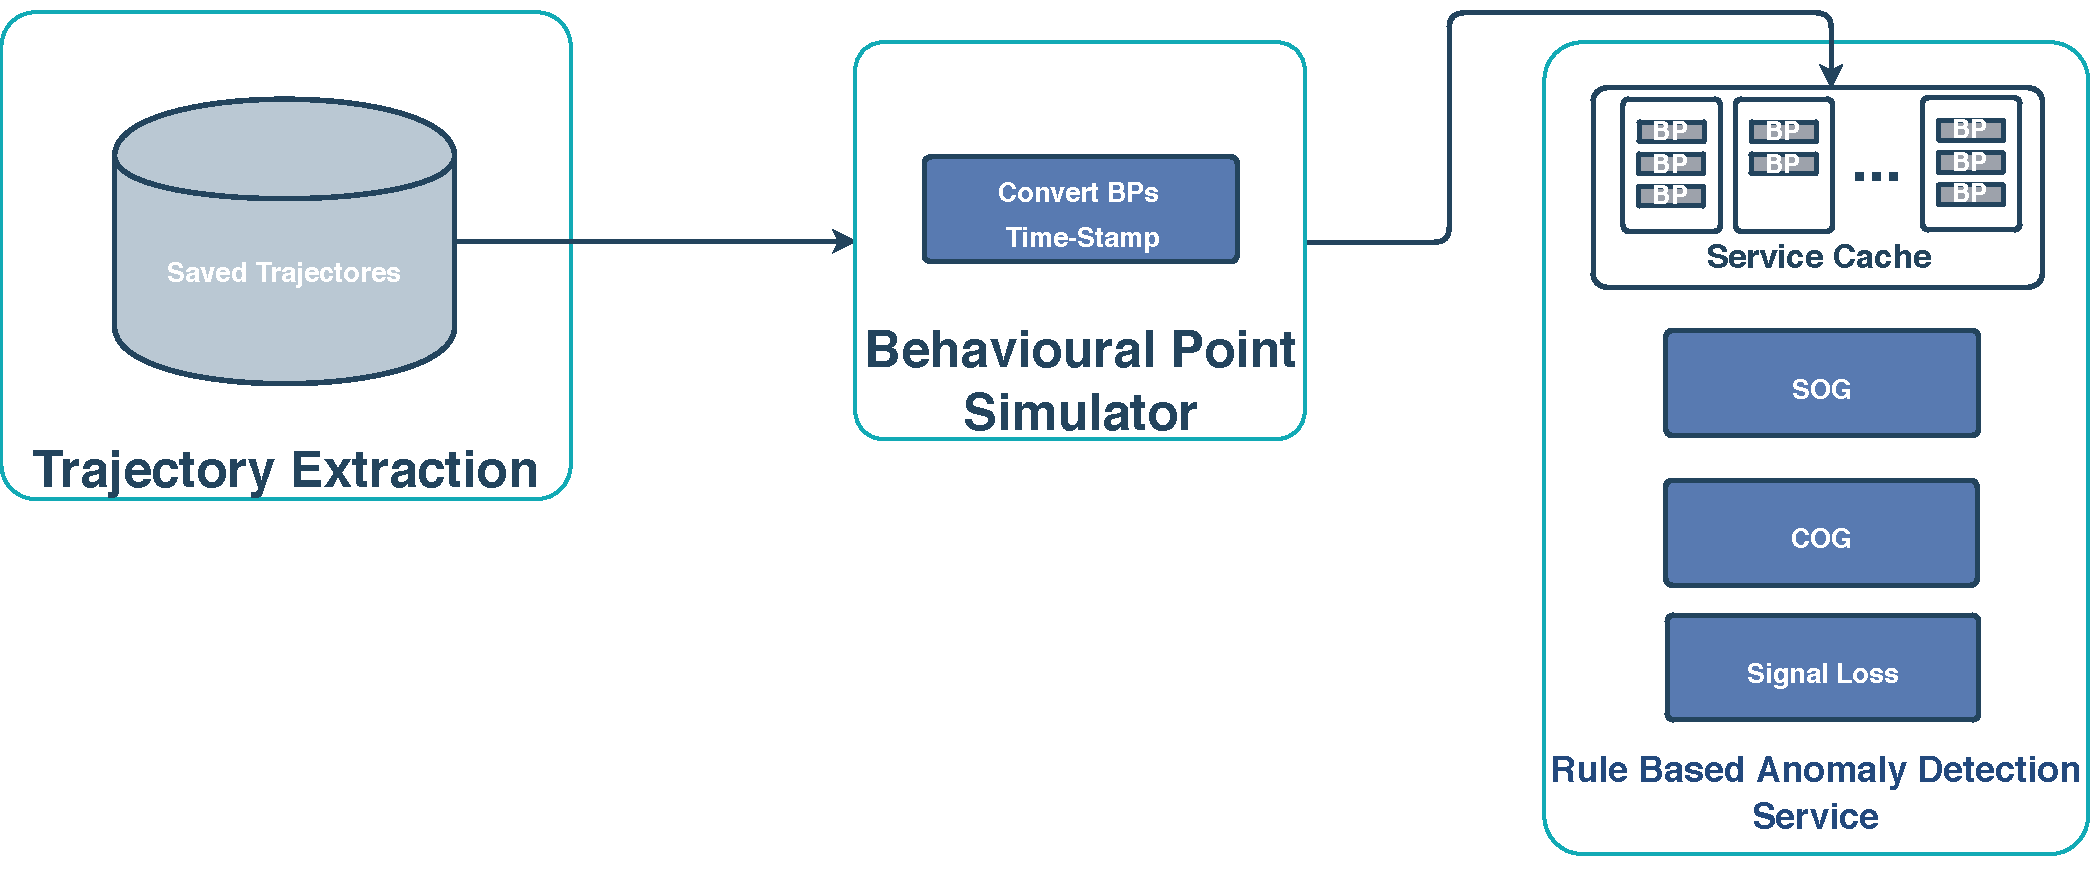
\includegraphics[width=\textwidth]{figures/Ch5/SRM-Exp-Simulator.pdf}
    \caption{BPs Simulator.}
    \label{fig: 5 BPs Simulator}
\end{figure}

The simulator worked by setting the a \textbf{Initial-Simulated-Time} as if it was the current Time. This time was the first time-stamp of the stored $BPs$. Based on this \textbf{Initial-Simulated-Time}, the following $BPs$ would be sent based on the time difference from this \textbf{Initial-Simulated-Time}. As it would be impractical to wait 5 days for the simulation of the reception of this data, the developed simulator was implemented with a \emph{speed up factor}. This some what allowed us to replicate the real reception of the same data, while simultaneously analysing the results of different rules.

\iffalse
Thus, using the $BPs$ simulator additional rules could be applied with the same data, thus gaining insight on the generated anomalies. 

which were considered anomalous for $R1$ were not considered in $R3$, which would be the same as defining a new rule that would be $COG.diff>25~and~Time$ which we gonna name \textbf{$R4$}.
If $R4$ would be applied on the same data, only   

As new $BPs$ were being created by the MAD-F, from the NMEA feed, the RB-ADS module was generating anomalies, based on the rules previously defined. This in the end generated a total of XXX anomalies, which we detail in Table XXX.

\todo[inline]{SEE IF I WANT TO TALK ABOU THE MEADIAN TIME ETC ETC...}

was acquiring messages from the NMEA feed, the
we injected the resulting $BPs$ from the Experiment~\ref{section: Experiment Data} in the RB-ADS module. Therefore this experiment was not conducted using the real-time data NMEA feeds. If the feed would be used,  we would loose control of the incoming data, which would make this experiment not possible to replicate.

For this Experiment the \textbf{Initial-Simulated-Time} was set first received $BP$ from the Experiment~\ref{section: Experiment Data}, which was XXXXXXTODOXXXXXX.  

As it would be not practical waiting 5 days for this Experiment, we 
Thus, we ran RB-ADS with the simulator setted to a speed of X. 

The RB-ADS was then executed with the set of rules represented under in Table and with the RB-ADS parameters represented in Table~\ref{Table: 5 exp. RB-ADS rules}.


With the parameters described above, we generated a sum of XXX anomalies from the 3 rules used, as detailed in table XX. 
\fi

\section{Anomaly Detection Service Experiment}
\emph{ADS Experiment} for this current work represents our validation process of the developed offline AD functionalities. The steps towards this experiment were similar to the Experiment~\ref{section: RB-ADS Experiment}. As this module was developed to access more complex anomaly detection methods by the use of batches of historical data. We did not conduct this experiment same data as presented in~\ref{section: Experiment Data} or had a similar approach as for the Experiment~\ref{section: RB-ADS Experiment}.
As we already had preconceived knowledge of the dataset which we used in our initial data-analysis (Section~\ref{section: Data Analysis}). We conducted this Experiment with the same dataset, as it in fact represented an huge batch of historical data.
presented an huge batch of data. 

Before performing of the \emph{ADS Experiment} itself, the raw dataset was injected in the MAD-F as a single batch of data. This transformed a the historical AIS dataset into a normalised set of $BPs$, which was kept stored in \emph{Trajectory Data-Base}. What is to note is that if this group of $BPs$ were to be stored as files, these files would be nearly 5 GB(if stored as .csv type files).
As the transformation of the dataset in $BPs$ made the dataset pass through the "pre-processement" pipeline. This cleaned the whole dataset which was of initially 18,84 Million rows (AIS messages), from 4555 different Vessel, into approximately 17,10 Million $BPs$.
After the $BPs$ were store as trajectories, and additional "manual" filtering was done. We filtered the trajectories with a size inferior of 100 $BPs$. This filtering only slightly reduced the number of total $BPs$ considered for this experiment to 17,06 Million, although the number of considered Vessels was dramatically reduced to 1588 Vessels.

The ADS experiment was divided into two Sections. The first section presents the results obtained for the Vessel Rendezvous detection, and the second section presents the results for the Incoherent Navigational Status and Time Space incompatibility. The results are presented as the generated anomalies from the ADS module. From each subsection we present an explanatory analysis of the generated anomalies.  

\subsection{ADS - Rendezvous Experiment}
\label{subsection: ADS - Rendezvous Experiment}
This subsection, shows the results and our analysis of the results obtained from the Rendezvous sub-experiment. This sub-experiment was conducted on the the historical batch of data which was described above. The Rendezvous detection, as any other module of the proposed MAD-F was developed to be configured with the set of parameters most adequate for the situation which would be deployed. This choice of parameters in any real scenario would be done by Maritime Experts. Although for the sole purpose of this Experiment, the choice of parameters was done by us. This Experiment was conducted with four different sets of configurations(Table~\ref{Table: 5 ADS Rendezvous input paramenters}).

\begin{table}[H]
\centering
\caption{Anomaly Detection Service - Rendezvous input parameters.}
\label{Table: 5 ADS Rendezvous input paramenters}
\begin{tabular}{@{}cccc@{}}
\toprule
Rendezvous Parameter & BPs & Time-Window & Distance Threshold \\ \midrule
C1 & 17.1M & 10 min. & 50 yards \\
C2 & 17.1M & 2 min. & 50 yards \\
C3 & 17.1M & 10 min. & 10 yards \\
C4 & 17.1M & 2 min. & 50 yards \\ \bottomrule
\end{tabular}
\end{table}

The four different set of configurations were chosen in order to demonstrate the rendezvous anomaly detection capabilities. By varying the configuration the rendezvous detection can either be done in a more precise way, or in a more efficient way. The variation of \emph{Time-Windows} directly impacts the granularity of the detection and the variation of the \emph{Distance Threshold} impacts the proximity the vessels were to each other. In the Table~\ref{Table: 5 ADS Rendezvous results} we present the results obtained with the configurations presented above.

\begin{table}[H]
\centering
\caption{Rendezvous experiment results, with the variation of the configuration parameters. }
\label{Table: 5 ADS Rendezvous results}
\begin{tabular}{@{}cccc@{}}
\toprule
Parameters & Rendezvous Detected & Time Groups & Time Elapsed (aprox.) \\ \midrule
C1 & 35,667 & 131,760 & 50s \\
C2 & 120,773 & 26,352 & 4min. \\
C3 & 5,704 & 131,760 & 2min. \\
C4 & 18,993 & 26,352 & 40s \\ \bottomrule
\end{tabular}
\end{table}

From the results presented above, the first thing we noticed was that the number of occurrences was larger than expected. Regarding the variation of configurations what was found out, was that the variation of distance threshold impacts the number of possible rendezvous detentions, which was expected.
What was not expected was the number of occurrences increasing with the decrease of the time-groups sizes. 
Although, after analysing the results, this results did exactly what the method was developed for. As for this work, we considered an anomaly to be a single instance in time, and not the time group of which the anomaly had occurred. When considering lower time-groups sizes if two vessels had report twice in same position, two anomalies would be created. For the purpose of this analysis, and in order to mitigate this duplication of technically the same anomaly, thus gaining insight of how many rendezvous had occurred. We grouped the anomalies, therefore, if the anomalies were generated by the same group of vessels, in consequent time-groups they would be considered the anomaly with same with a larger duration. 
What was discovered from this grouping of consequent anomalies was that, with the configuration parameters \textbf{C4}, only \textbf{75} combinations of two vessels generated rendezvous anomalies. Although each combination of vessels generated multiple times rendezvous occurrences, with some combinations generating up to \textbf{7,436} times.

After analysing the frequency of occurrence, we analysed the location where the possible rendezvous had occurred. This led us to conclude that most of the detected rendezvous occurrences occurred nearby port.
As the only truly way to validate the results was by providing this results to a Maritime Officer which could not be achieved for the sole purpose of this present work. We decided to represent the Rendezvous occurrences which we detected on a distance of above 2 Km of the closest Port, thus creating a footprint of the possible Rendezvous occurrences for the whole dataset. A similar analysis is done by the authors in~\cite{Miller2018IdentifyingBehavior}. 

In Figure~\ref{fig: Chapter 5 Rend2Mapsr}, we present the a visual representation of the locations where the Rendezvous anomaly occurrence, from the area near the port of Brest(France). By displaying only the rendezvous events that occurred 2Km away from the closest port, the number of rendezvous occurrences is significantly reduced, it is possible to visualise in Figure~\ref{fig: Chapter 5 Rend2Mapsr}(Right). Nevertheless, as the a port for this work was considered as a single point, and a port can be way larger than just a single point. Filtering by the distance to port, by just considering as a point can cause a occurrence to not be filtered as sill in port. This problem will be addressed for Future Work.


\begin{figure}[H]
	\centering
	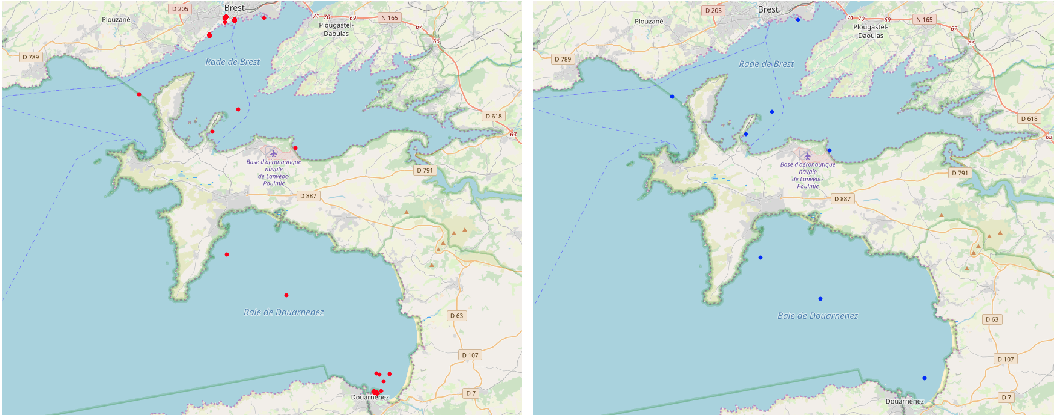
\includegraphics[width=\textwidth]{figures/Ch5/ThesisExpRend.pdf}
    \caption{Rendezvoused results, on the left no distance filter is applied and in right 2Km distance to port is applied.}
    \label{fig: Chapter 5 Rend2Mapsr}
\end{figure}


%As vessels being close to each-other inside a port is not anomalous, and brings no value to the Maritime Officers, we analysed the distance to port from the detected rendezvous occurrences. 
%In TableXXXX%~\ref{Table: 5 Distance to Port Rendevouz} we present the distance distribution, from the.
%The occurrences based in the Distance to Port, show that 20\% of the detected Rendezvous occurrences occur at Distance less than 500 Meters to Port. 

\subsection{ADS - Time Space Incompatibility Experiment}
\label{subsection: ADS - Time Space Incompatibility Experiment}
The time space incompatibility Experiment, serves for this present work as a Experiment in which we analyse the results from the ADS time-space incompatibility anomaly detection module. In order to achieve this, we took two different analysis for the this Experiment. First we analyse the overall anomalies generated, by varying the input parameters of this service. Secondly, as this service represents a some what first approach towards a vessel positional estimation, we applied the implemented linear estimation to the vessel trajectory, which was presented in~\ref{subsection: 4 Time-Space Incompatibility}, to a single trajectory which was presented in~\ref{subsection: Trajectory Definition}.

By following a similar approach as the one presented for the rendezvous Experiment, we used the historical batch of data previously described also for the detection of the space time incompatibility. As the \emph{Distance Factor Threshold}, is the configuration parameter for this specific anomaly detection, and it should be configured by a Maritime Expert depending on the scenario. For this Experiment we varied the $dft$ and analysed the results.  In Table~\ref{Table: 5 Time Space} we present the number of occurrences of the what was interpreted for this present work as the \textbf{AR5}(presented in Section~\ref{section: Framework Requirements}). 

\begin{table}[H]
\centering
\caption{Time space incompatibility occurrences, by varying the $dft$, and comparing with the $BP$ time shift.}
\label{Table: 5 Time Space}
\begin{tabular}{@{}cccccc@{}}
\toprule
Distance Factor Threshold & Delta Time & \textless{}2min. & \textless{}5min. & \textless{}15min. & \textgreater{}15min. \\ \midrule
500m & 6,581 & 391 & 866 & 1,978 & 4,559 \\
1km & 4,289 & 187 & 229 & 685 & 3,569 \\
2.5km & 2,373 & 53 & 53 & 95 & 2,257 \\
5km & 1,353 & 38 & 38 & 40 & 1,295 \\ \bottomrule
\end{tabular}
\end{table}

What was expected from this anomaly detection, was that the number of detected anomalies would increase with the decreasing of $dft$, this was confirmed by our Experiment. From this conclusion we further analysed this results by comparing the number of detected anomalies with the time shift from the previous $BP^{T-1}$, as we described in Section~\ref{subsection: ADS - Time Space Incompatibility Experiment}.
What is possible to analyse is the correlation from the time elapsed with the number of detected time space incompatibility occurrences. Thus, an Signal Loss Anomaly would also trigger a time space incompatibility anomaly.

Additionally for this Experiment, we applied the enriched Linear Estimation Equation which was presented in Section~\ref{subsection: 4 Time-Space Incompatibility} to a single trajectory of a Vessel, as we present under in Figure\ref{fig: Chapter 5 SMM linear estimation}. 
\begin{figure}[H]
	\centering
	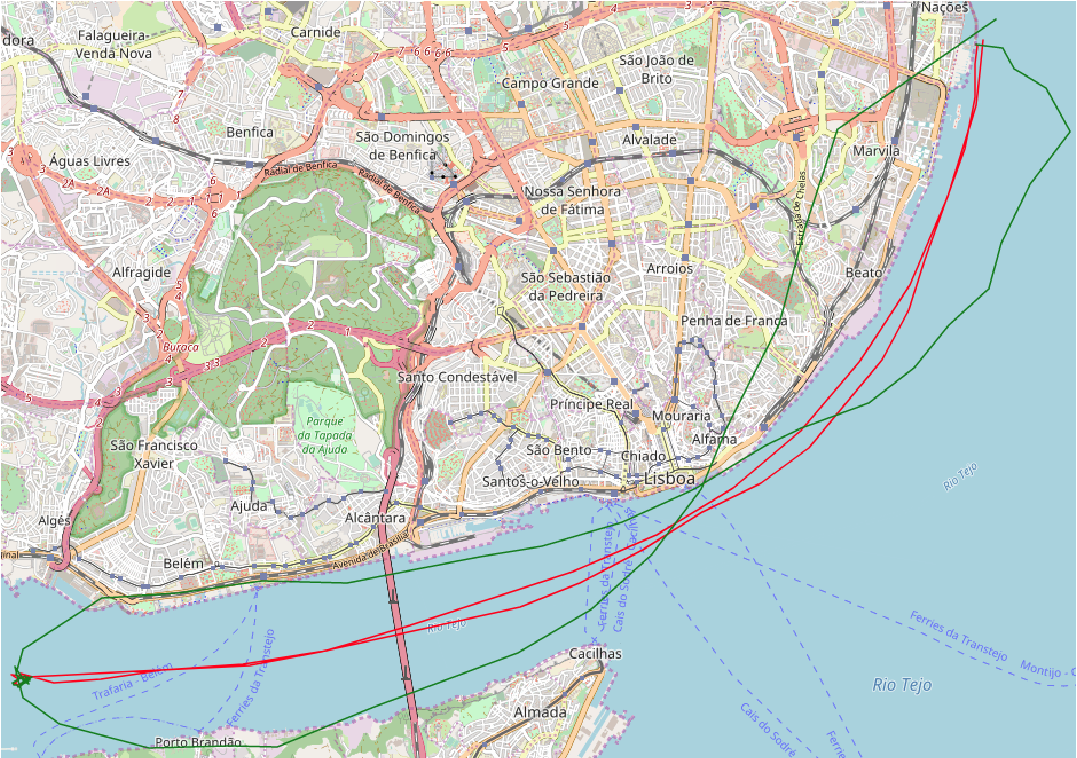
\includegraphics[scale = 0.75]{figures/Ch5/SMM_Estimation_Croped.pdf}
    \caption{Linear Trajectory estimation (Green), applied to the Vessel Trajectory (Red) presented in Section~\ref{subsection: Trajectory Definition}.}
    \label{fig: Chapter 5 SMM linear estimation}
\end{figure}
For any historical trajectory it is possible to know where the was each for every transmission, by calculating the haversine distance between the estimated position at $T^{-1}$ and the actual vessel position at time $T$. This distance represents the distance estimation error. For this trajectory which length was of $138$ $BPs$, the mean distance estimation error was of \textbf{361 meters}. This result for this trajectory were suboptimal, as firstly a Vessel position should never be estimated to be in land, and secondly this specific trajectory had $98$ $BPs$ with a reported $SOG$ under 1knot. Despite all, the presented sub-esperiment, serves as a baseline, for the implementation of more advanced trajectory estimation mehtods as we will discuss in Future Work,~\ref{chapter:Chapter6}.

\subsection{ADS - Navigational Status Validation Experiment}
\label{subsection: ADS - Navigational Status Experiment}
The Navigational Status Validation Experiment, was conducted with similar approach as the Experiment~\ref{subsection: ADS - Rendezvous Experiment}.
This experiment, started with the analysis of the usage frequency of each Navigational Status, as it is presented under in Table~\ref{Table: 5 Status Counts}.
\begin{table}[H]
\centering
\caption{Navigational Status Counts, where the \% is rounded to two decimal places.}
\label{Table: 5 Status Counts}
\begin{tabular}{@{}ccc@{}}
\toprule
Navigational Status & Count & Count(\%) \\ \midrule
0 & 8,895,694 & 52\% \\
15 & 5,334,804 & 31\% \\
5 & 1,030,712 & 6\% \\
7 & 1,012,271 & 6\% \\
3 & 391,141 & 2\% \\
1 & 177,925 & 1\% \\
8 & 71,664 & 0.0\% \\
2 & 23,306 & 0.0\% \\
6 & 14,955 & 0.0\% \\
4 & 62 & 0.0\% \\ \bottomrule
\end{tabular}
\end{table}

In Table~\ref{Table: 5 Status Counts} what is possible to notice is that the distribution of the reported navigational status is extremely skewed. With approximately $83\%$ of all the analysed $BPs$ were reported as either Status 0(Under Way Using Engine) or 15(Default State). 
Despite this skewed distribution, the experiment was still conduced for the statuses that were quantifiable in a stopped or moving expert label, which was explained in Section~\ref{subsection: 4 Navigational Status Validation}. 
This ultimately reduced the $BPs$ which were evaluated by this experiment. Nevertheless the experiment was conducted with $10.1$ Million $BPs$, where the results under in Table~\ref{Table: 5 Status Results}.
%which limited reduced the  Experiment and as described in Section XX, we validated the Navigational Statuses that could be described in a Stopped or Moving kinematic label.  The skewed distribution of the Navigational Status reported in this Data-Set, allowed this validation to be done for the major part of this Data-Set. We were able to validate, validate XXMILION MESSAGES XXPERCENTAGE...
  
\begin{table}[H]
\centering
\caption{Results for Navigational Status Validation Experiment, with the Stopped or Moving approach. }
\label{Table: 5 Status Results}
\begin{tabular}{@{}lllc@{}}
\toprule
Navigational Status & Count & Incoherent Count & Incoherent \% \\ \midrule
0 (using engine) & 8,895,694 & 5225362 & 58.74\% \\
1 (at anchor) & 177,925 & 54,085 & 30.40\% \\
5 (moored) & 1,030,712 & 246,430 & 23.91\% \\
6 (aground) & 14,955 & 2,091 & 13.98\% \\
8 (sailing) & 71,664 & 24,607 & 34.34\% \\
Total & 10,190,950 & 5,552,575 & 54.49\% \\ \bottomrule
\end{tabular}
\end{table}

From the results presented above, it is clear that the major part of the used Navigational Statuses were reported wrongly. Similar results were found in~\cite{Machado2019VesselOutliers}, using a different dataset. A possible reason for such high number of miss used navigational status, might be justified by the fact that the Navigational Status is set by the crew on the AIS device. 
Although to try to better understand this results we started by analysing the areas where the miss-use of navigational status would occur. This analysis is presented in the form of a density plot, which was done using the same packages, as in Experiment~\ref{section: Experiment Data}.

\begin{figure}[H]
	\centering
	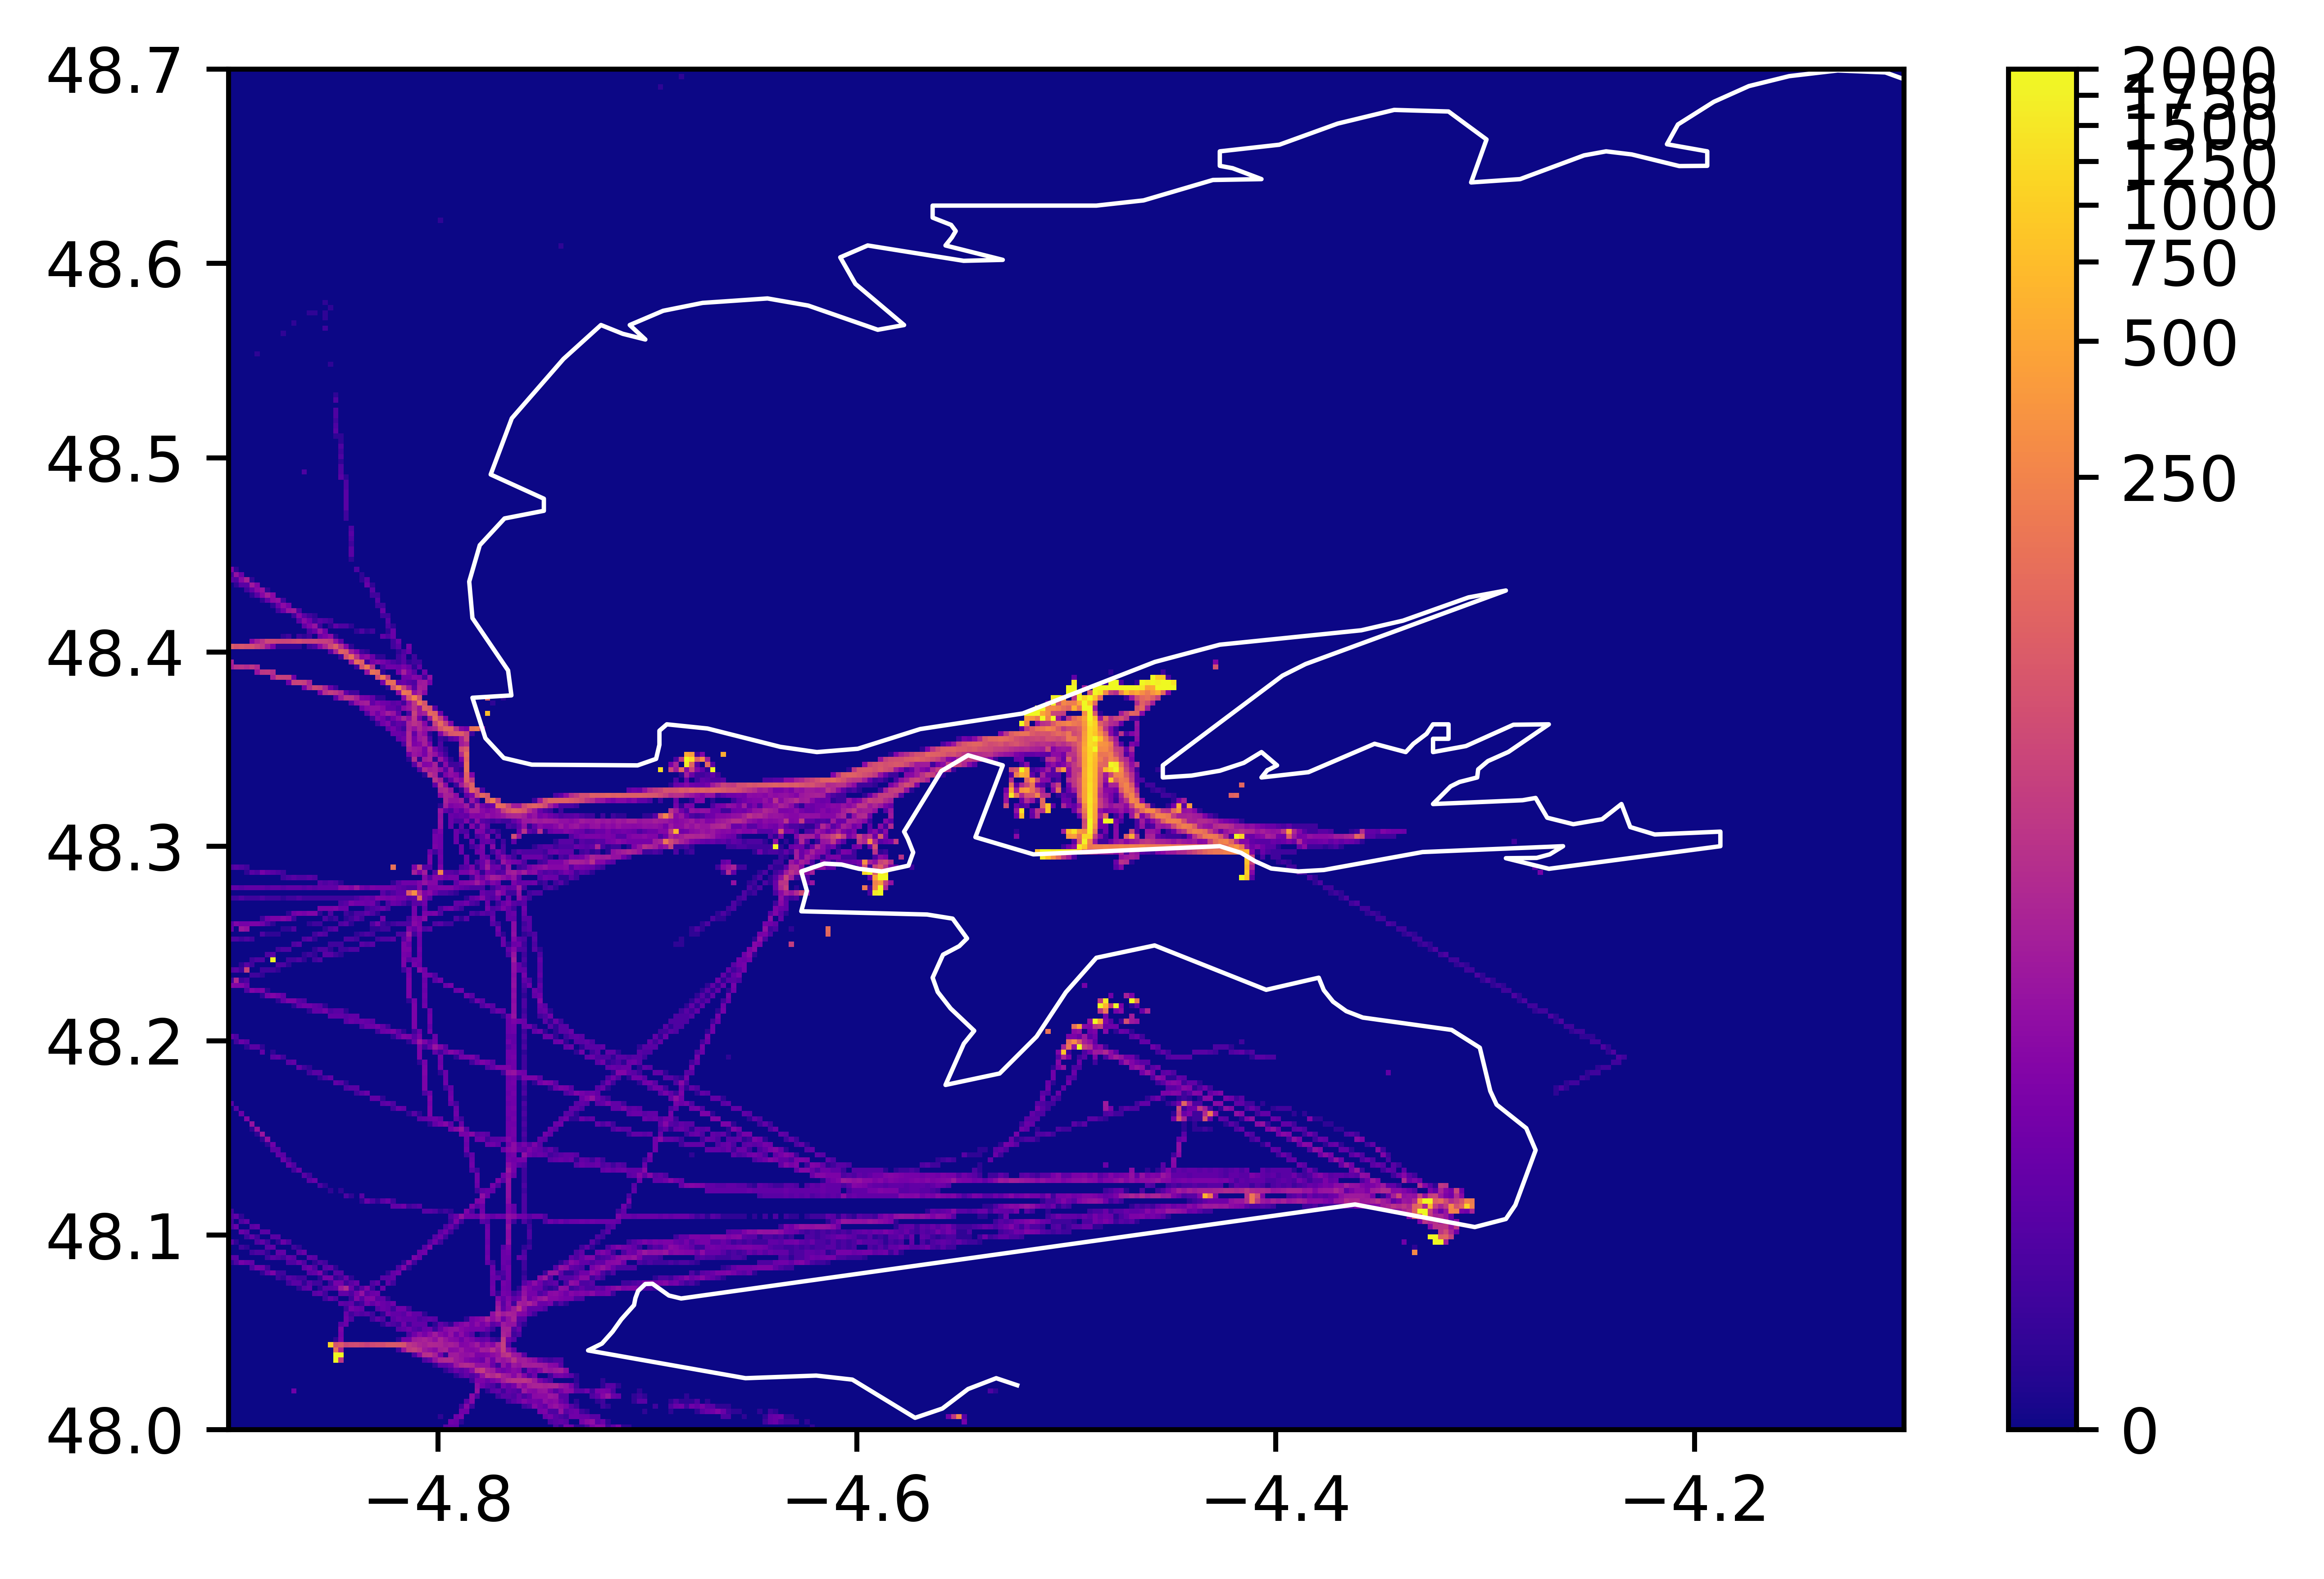
\includegraphics[width=\textwidth]{figures/Ch5/ThesisExpStatusDensityZoom.png}
    \caption{Density map, with all the 5,5M occurrences of wrong Navigational Status.}
    \label{fig: 5 Exp StatusDensityMap}
\end{figure}

What we were able to notice in Figure~\ref{fig: 5 Exp StatusDensityMap}, is that the high density areas where the Navigational Status is reported wrongly, are areas really close to port. As the AIS navigational status needs to be changed each time the vessel arrives at port. This led us to believe that the crew members "forgets" to change the navigational status, while in port. Which is then represented on the data, as the Vessel being stopped on port for long periods of time with the navigational status 0(under way using engine). 

\subsubsection{ADS - Fishing Status Validation Experiment}
\label{subsection: ch5 fishing validation}
Fishing status validation is a sub-Experiment related to the Experiment presented above. As to the best of our knowledge there are no current \emph{public} classified fishing trajectories datasets, the approach taken to validate the usage of this specific status was merely by our analysis. What we done for this sup-Experiment, was the usage of the already pre-defined Gaussian Mix Model presented in Section~\ref{subsection: Fishing Activity Detection}. The model was applied on the sub-set of $BPs$ which had the AIS navigational status reported as \textbf{7 - engaged in fishing}. Despite the acknowledged generalisation and the limited validation of the presented model the presented results serve as our first steps towards the implementation of a MAD-F \emph{fishing detection module}. This will be discusses for future work in Chapter~\ref{chapter:Chapter6}. 

For this sub-experiment we first provide an exploratory analysis of the reported $BPs$ and what would be expected to be reported from fishing vessels. From approximately 3 million $BPs$, transmitted by the fishing vessels (vessel type 30) only about 30\% was in fact transmitted with the navigational status 7(engaged at fishing), as the rest half of them were reported with the default AIS status and as we present in Table~\ref{Table : 5 Fishing Status Counts}. 

\begin{table}[H]
\centering
\caption{Fishing Vessels, Navigational Status Counts, where the \% is rounded to two decimal places.}
\label{Table : 5 Fishing Status Counts}
\begin{tabular}{@{}ccc@{}}
\toprule
Navigational Status & Count & Count(\%) \\ \midrule
15 & 1,290,264 & 0.42 \\
7 & 919,515 & 0.30 \\
0 & 749,419 & 0.25 \\
3 & 37,092 & 0.01 \\
5 & 25,505 & 0.01 \\
8 & 6,394 & 0.00 \\
2 & 2,164 & 0.00 \\
6 & 2,055 & 0.00 \\
1 & 19 & 0.00 \\ \bottomrule
\end{tabular}
\end{table}

We further analysed the transmitted navigational status by analysing, if weather any other vessels had transmitted the engaged at fishing navigational status. As presented under in Table~\ref{Table : 5 Fishing Vessel Type}, we noticed that approximately 10\% of the reported $BPs$ were in fact transmitted by other types of Vessel.

\begin{table}[H]
\centering
\caption{Vessel types which had reported the engaged at fishing navigational status.}
\label{Table : 5 Fishing Vessel Type}
\begin{tabular}{@{}lcl@{}}
\toprule
Vessel Type & Vessel Type Nº & Count \\ \midrule
Fishing Vessel & 30 & 919,515 \\
Other & 90 & 92,576 \\ \bottomrule
\end{tabular}
\end{table}

After this initial analysis, we applied a fishing navigational status validation, by classifying the reported engaged at fishing $BPs$ into a steaming (high speed) or fishing (low speed). From this results we further analyse this classification by comparing this results with the mean speed average, from each group, as we present under in Table~\ref{table: ch5 GMM}.

\begin{table}[H]
\centering
\caption{Fishing, not Fishing classification using the Gaussian Mix Module.}
\label{table: ch5 GMM}
\begin{tabular}{@{}lcc@{}}
\toprule
Label       & Count     & Mean SOG \\ \midrule
Fishing     & 1,552,816 & 6.89   \\
Not Fishing & 1,487,490 & 2.60   \\
Total       & 3,040,306 & 8.72   \\ \bottomrule
\end{tabular}
\end{table}

\section{Marisa Validation Trials}
\label{Section: 5 Marisa Validation}

This section presents how the validation of the developed MAD-F will be processed. The evaluation presented above serves as our own analysis and examination of the results produced by the developed MAD-F. Even though the present work was developed in a highly collaborative spirit, the results used must be evaluated under the project context in order for any method to be truly validated. In \textsc{Marisa}, this is achieved by including the different partners into what was defined in the project as \textbf{Trials}. A Trial represents a defined operational scenario where the project end-users will test the developed \textsc{Marisa} services. Despite the intermediate validation procedures applied throughout this work, the ultimate validation of the developed MAD-F is solely conditional on the performance 
of the project trials. By aggregating the users by region of activity, five different trials were defined for the \textsc{Marisa} Project and they will take place until the end of $2018$. \textsc{Inov} will be present in three of these Trials. For 
the purpose of the present work, we shall describe the Trial for which \textsc{Inov} contributed the most for the preparation of the Iberian Trial. The Iberian Trial will be conducted by the Portuguese Navy and the Spanish Guarda Civil, and will involve \textsc{Inov} and numerous other project partners. This will occur during the first fortnight of November, around the region of the Algarve (Portugal), as shown in Figure~\ref{fig: 5 TrialArea}.  

\begin{figure}[H]
	\centering
	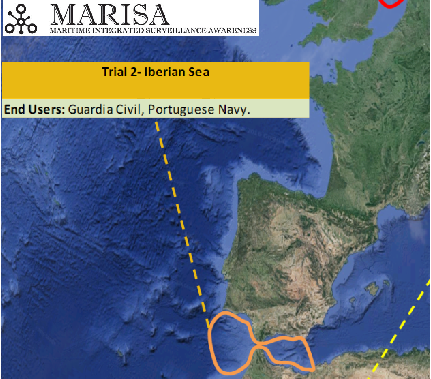
\includegraphics[scale=1.4]{figures/Ch5/IberainTrial.pdf}
    \caption{\textsc{Marisa} Iberian Trial operational area.}
    \label{fig: 5 TrialArea}
\end{figure}

\textsc{Inov} was present in previous meetings with the Portuguese Navy, where the overall execution of the Iberian Trial was discussed. Within the scope of this work's efforts, we are currently ready and able to correlate the Trial activities with the effective validation of the Services and thus the MAD-F. The Iberian Trial will be conducted with real assets, including military vessels from both the Portuguese Navy and the Spanish Guarda Civil, the end-users of this project. Maritime Agents will perform a somewhat choreographed set of vessel manoeuvres able to trigger anomalies. In Table~\ref{Table: Ch5 Trial}, we present the choreography exercise, which will be performed by the Maritime Agents, and how they are correlated with the developed  MAD-F (more specifically by correlating with the Anomaly Requirements which were presented in Section~\ref{section: Framework Requirements}). 
\begin{table}[H]
\centering
\caption{Part of the Choreography conducted for the Iberian Trial. Where V1 and V2 represent a vessel from each end-user, and OC the Operation Control.}
\label{Table: Ch5 Trial}
\resizebox{\textwidth}{!}{%
\begin{tabular}{@{}lll@{}}
\toprule
Provided Description & Choreography & Remarks \\ \midrule
COMMCHECKS & \begin{tabular}[c]{@{}l@{}}at 1000:\\ - OC - communications checks.\end{tabular} &  \\ \midrule
\begin{tabular}[c]{@{}l@{}}TRANSIT TO \\ HIGH SEA\end{tabular} & \begin{tabular}[c]{@{}l@{}}at 1100:\\ - V1 - turns to portside 40º, heading to 140º\end{tabular} &  \\ \midrule
\begin{tabular}[c]{@{}l@{}}TRANSIT TO \\ HIGH SEA\end{tabular} & \begin{tabular}[c]{@{}l@{}}at 1130:\\ - V1 - turns to starboard side 40º, heading to 180º\\ - V1 - increases speed to 25KTS and maintains for 10min.\end{tabular} & \begin{tabular}[c]{@{}l@{}}Aim is to detect Change in  \\ Course Over Ground (COG) and\\ Speed Over Ground (COG).\end{tabular} \\ \midrule
\begin{tabular}[c]{@{}l@{}}TRANSIT TO \\ HIGH SEA\end{tabular} & \begin{tabular}[c]{@{}l@{}}at 1200:\\ - V1 - Turns the AIS System from 1200 to 1220.\\ - OC - Checks if it is detected a change in the AIS System.\end{tabular} & \begin{tabular}[c]{@{}l@{}}Aim is to detect \\ non-broadcasting (AIS)\end{tabular} \\ \midrule
RENDEZVOUS & \begin{tabular}[c]{@{}l@{}}at 1230:\\ - V2 - approaches towards P1(TBD).\\ - V2 - approaches towards P1(TBD).\end{tabular} &  \\ \midrule
RENDEZVOUS & \begin{tabular}[c]{@{}l@{}}at 1300:\\ - V1 - stops at P1 for more than 5min.\\ - V2 - stops at P1 for more than 5min.\end{tabular} & \begin{tabular}[c]{@{}l@{}}Aims to detect the \\ repeated rendezvous \\ of 2 Vessels.\end{tabular} \\ \midrule
\begin{tabular}[c]{@{}l@{}}TRANSIT ALONG \\ SIDE COASTLINE\end{tabular} & \begin{tabular}[c]{@{}l@{}}at 1400:\\ - OC - manipulates the V1 and V2 AIS signal.\\ - V1  - heads to port.\\ - V2  - heads to port.\end{tabular} & \begin{tabular}[c]{@{}l@{}}Aims to detect \\ Incoherent Position and \\ Navigational Status.\end{tabular} \\ \bottomrule
\end{tabular}%
}
\end{table}

The choreography exercise just detailed, within the greater scope of the Iberian Trial, will test conclusively the capabilities of our methodologies. It is worth mentioning that a large portion of Data Science projects suffer from either absent or weak validation stages. This project, in turn, relies on actual, verifiable validation schemes which were devised and coordinated appropriately, given the excellent collaboration links provided by the \textsc{Marisa} project.